\section{Введение}

\graphicspath{{parts/guides/1_introduction/images/}}

\subsection{Рекомендуемые к использованию инструменты}

Для освоения курса разработки оконных приложений для настольных систем Windows с помощью технологии WPF рекомендуется использовать IDE (интегрированную среду разработки) \textbf{Visual Studio Community 2017} с установленными расширениями \textbf{JetBrains ReSharper Ultimate} и \textbf{MVVM Light Toolkit}.

\subsection{Обзор технологии WPF}

Технология WPF (Windows Presentation Foundation) является часть экосистемы платформы .NET и представляет собой подсистему для построения графических интерфейсов для настольных систем Windows.

Одной из особенностей является то, что WPF использует расширяемый язык разметки для приложений (XAML), чтобы предоставить декларативную модель для программирования приложений. XAML основан на языке XML. Таким образом возможно создание пользовательского интерфейса, используя декларативное объявление и/или код на языке C\texttt{\#}.
\todo{Подумать над оформлением}


\newpage
\subsection{Создание проекта}
Давайте начнем изучение нашего курса с создания проекта приложения.

\begin{enumerate}
    \item Откройте \textbf{Visual Studio} и выберите \textbf{файл} (\textbf{File}) > \textbf{Создать} (\textbf{New}) > \textbf{Проект} (\textbf{Project}).
    \item В разделе \textbf{установленные} (\textbf{installed}) выберите подраздел \textbf{Visual C\texttt{\#}}
    \item Затем выберите пункт \textbf{Приложение WPF (.NET Framework)} / \textbf{WPF App (.NET Framework)}
    \item В нижней части окна вы можете указать основные параметры Вашего приложения
    \item Укажите \textbf{имя} (\textbf{name}) приложения (Например, \textit{HelloWorldApp}) и \textbf{путь} (\textbf{location}) для его сохранения
    \item \textbf{Имя решения} (\textbf{solution name}) можно оставить таким же как и \textbf{имя} приложения
    \item Рекомендуется выбрать платформу \textbf{.NET Framework 4.7.1}
    \item Отметьте пункт \textbf{Создать каталог для решения} (\textbf{Create directory for solution})
    \item Если вы хотите использовать систему контроля версий \textbf{Git}, то отметьте пункт \textbf{Добавить в систему управления версиями} (\textbf{Create new Git repository})
    \item Нажмите кнопку \textbf{OK}
\end{enumerate}

\begin{figure}[H]
\centering
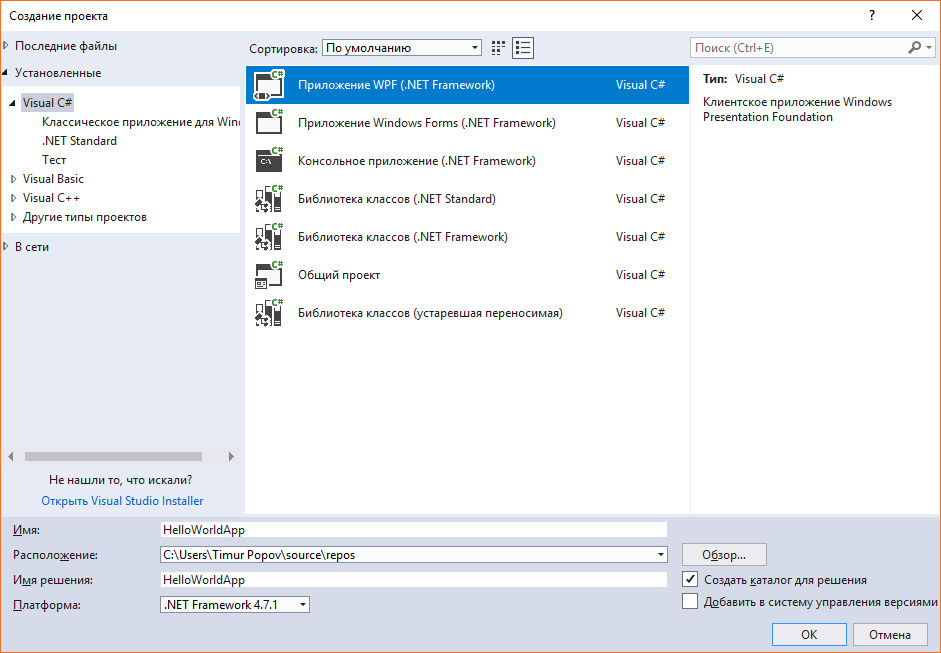
\includegraphics[width=1\textwidth]{introduction_create_project.png}
\end{figure}

\newpage
По умолчанию \textbf{Visual Studio} открывает создает и открывает нам два файла: файл декларативной разметки интерфейса \path{MainWindow.xaml} и файл связанного с разметкой кода \path{MainWindow.xaml.cs}. Файл \path{MainWindow.xaml} имеет два представления: визуальное — в режиме \textbf{WYSIWIG} отображает весь графический интерфейс данного окна приложения, и под ним декларативное объявление интерфейса в \textbf{XAML}. Если мы изменим декларативную разметку, например, определим там кнопку, то эти изменения отображаться в визуальном представлении.

\begin{figure}[H]
\centering
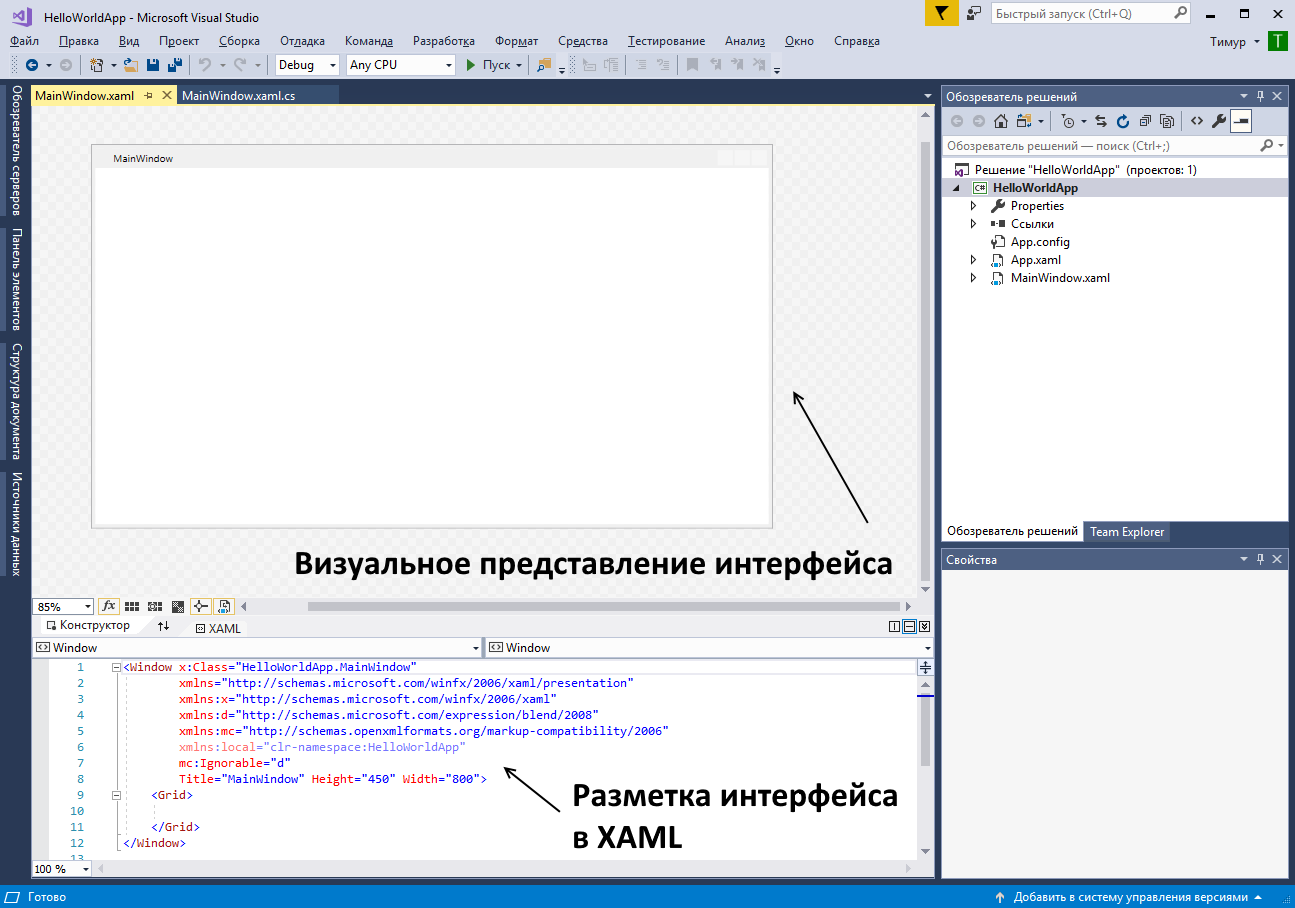
\includegraphics[width=1\textwidth]{introduction_project.png}
\end{figure}

\newpage
\subsection{Знакомство с базовой структурой WPF приложения}

Главным файлом в проекте является \path{App.xaml} и связанный с ним файл кода \path{App.xaml.cs} — это глобальные файлы для всего приложения, определяют его параметры и ресурсы. Так же там указан файл, определяющий главное окно приложения, которое будет открываться при запуске. Это происходит в следующей строке

\begin{minted}{xml}
StartupUri="MainWindow.xaml"
\end{minted}

то есть в данном случае, когда мы запустим приложение, будет создаваться интерфейс из файла \path{MainWindow.xaml}. 

У каждого файла \path{*.xaml} есть парный ему файл \path{*.xaml.cs}, который ещё называется \textbf{Code-Behind}. В нем сокрыта вся внутренняя структура, что позволяет ускорить написание кода и упростить поиск ошибок.

Так же вы обнаружите файл \path{App.confg}, который отвечает за настройку среды CLR и дополнительные параметры Вашего приложения.

\subsection{Основы XAML} \label{XAML_basics}
XAML (eXtensible Application Markup Language) — язык разметки, используемый для инициализации объектов в технологиях на платформе .NET. Применительно к WPF данный язык используется прежде всего для создания пользовательского интерфейса декларативным путем наподобие HTML в веб-программировании. Однако, сводить XAML к одному интерфейсу было бы неверно, и далее на примерах мы это увидим.

XAML — не является обязательной частью приложения, мы можем обходиться без него, создавая все элементы в Code-Behind. Однако использование XAML все-таки несет некоторые преимущества:

\begin{itemize}
\item Возможность отделить графический интерфейс от логики приложения.
\item Компактность, понятность. Код на XAML относительно легко поддерживать.
\end{itemize}

При компиляции приложения в Visual Studio код в XAML-файлах компилируется в бинарное представление, которое называется BAML (Binary Application Markup Language), а затем встраивается в финальную сборку приложения.

При создании нового проекта WPF он уже содержит файлы XAML. Создаваемый по умолчанию в проекте файл \path{MainWindow.xaml} будет иметь следующую разметку:

\begin{minted}{xml}
<Window x:Class="HelloWorldApp.MainWindow"
        xmlns="http://schemas.microsoft.com/winfx/2006/xaml/presentation"
        xmlns:x="http://schemas.microsoft.com/winfx/2006/xaml"
        xmlns:d="http://schemas.microsoft.com/expression/blend/2008"
        xmlns:mc="http://schemas.openxmlformats.org/markup-compatibility/2006"
        xmlns:local="clr-namespace:HelloWorldApp"
        mc:Ignorable="d"
        Title="MainWindow" Height="450" Width="800">
    <Grid></Grid>
</Window>
\end{minted}

Как и в структуре веб-страницы на HTML, здесь есть иерархия элементов. Элементом верхнего уровня является \mintinline{xml}{Window}, который представляет собой окно приложения. При создании других окон в приложении нам придется всегда начинать объявление интерфейса с элемента \mintinline{xml}{Window}.

Элемент \mintinline{xml}{Window} имеет вложенный пустой элемент \mintinline{xml}{Grid}, а также ряд свойств: \mintinline{xml}{Title}, \mintinline{xml}{Width}, \mintinline{xml}{Height}) — заголовок, ширину и высоту окна соответственно.

\subsubsection{Пространства имен XAML}

Чтобы задействовать элементы в XAML, мы подключаем пространства имен. Вторая и третья строчки в коде выше как раз и представляют собой пространства имен, подключаемые в проект по умолчанию. А атрибут \mintinline{xml}{xmlns} представляет специальный атрибут для определения пространства имен в XML.

Так, пространство имен \mintinline{xml}{http://schemas.microsoft.com/winfx/2006/xaml/presentation} содержит описание и определение большинства элементов управления. Так как является пространством имен по умолчанию, то объявляется без всяких префиксов.

\mintinline{xml}{http://schemas.microsoft.com/winfx/2006/xaml} — это пространство имен, которое определяет некоторые свойства XAML, например Name или Key. Используемый префикс \mintinline{xml}{x} в определении \mintinline{xml}{xmlns:x} означает, что те свойства элементов, которые заключены в этом пространстве имен, будут использоваться с префиксом \mintinline{xml}{x}, например \mintinline{xml}{x:Name} или \mintinline{xml}{x:Key}. Это же пространство имен используется уже в первой строчке 

\begin{minted}{xml}
x:Class="XamlApp.MainWindow"
\end{minted}

Здесь создается новый класс \mintinline{csharp}{MainWindow} и соответствующий ему файл кода, куда будет описываться логика для данного окна приложения.

Это два основных пространства имен. Рассмотрим остальные:

\mintinline{xml}{xmlns:d="http://schemas.microsoft.com/expression/blend/2008"} обеспечивает поддержку атрибутов в режиме дизайнера. Это пространство имен преимущественно предназначено для другого инструмента по созданию дизайна на XAML — Microsoft Expression Blend

\mintinline{xml}{xmlns:mc="http://schemas.openxmlformats.org/markup-compatibility/2006"} обеспечивает режим совместимости разметок XAML.

\mintinline{xml}{mc:Ignorable="d"} это выражение позволяет игнорировать парсерам XAML во время выполнения приложения дизайнерские атрибуты из пространства имен с префиксом \mintinline{xml}{d}, то есть из \mintinline{xml}{"http://schemas.microsoft.com/expression/blend/2008"}

\mintinline{xml}{xmlns:local="clr-namespace:HelloWorldApp"} пространство имен текущего проекта. Так как наш проект называется \path{HelloWorldApp}, то простраство имен называется аналогично. Через префикс \mintinline{xml}{local} возмжно получить XAML различные объекты, которые определены в проекте.

Важно понимать, что эти пространства имен не эквивалентны тем пространствам имен, которые подключаются при помощи директивы \mintinline{csharp}{using} в C\texttt{\#}. Так, например,

\mintinline{xml}{"http://schemas.microsoft.com/winfx/2006/xaml/presentation"} 

подключает сразу в проект следующие пространства имен:

\begin{minted}{csharp}
System.Windows
System.Windows.Automation
System.Windows.Controls
System.Windows.Controls.Primitives
System.Windows.Data
System.Windows.Documents
System.Windows.Forms.Integration
System.Windows.Ink
System.Windows.Input
System.Windows.Media
System.Windows.Media.Animation
System.Windows.Media.Effects
System.Windows.Media.Imaging
System.Windows.Media.Media3D
System.Windows.Media.TextFormatting
System.Windows.Navigation
System.Windows.Shapes
System.Windows.Shell
\end{minted}

\subsubsection{Элементы и их атрибуты}
Каждый элемент, как и любой элемент XML, должен иметь открытый и закрытый тег, как в случае с элементом \mintinline{xml}{Window}:

\mintinline{xml}{<Window></Window>}

Либо элемент может иметь сокращенную форму с косой чертой ("слэшем") в конце, наподобие:

\mintinline{xml}{<Window />}

Но в отличие от элементов XML каждый элемент в XAML соответствует определенному классу C\texttt{\#}. Например, элемент \mintinline{xml}{<Button>} соответствует \mintinline{csharp}{System.Windows.Controls.Button}. А свойства этого класса соответствуют атрибутам элемента \mintinline{xml}{<Button>}.

Например, давайте добавим в создаваемую по умолчанию разметку окна (она рассмотрена в \ref{XAML_basics}) менеджер компоновки \mintinline{xml}{StackPanel} (подробнее рассматривается в \ref{panel_definition}), а в него текстовое поле \mintinline{xml}{TextBox} и кнопку \mintinline{xml}{Button}. Для этого мы должны добавить в \mintinline{xml}{Grid} следующее

\begin{minted}{xml}
...
<Grid>
    <StackPanel VerticalAlignment="Center" Margin="50">
        <TextBox x:Name="MagicTextBox" />
        <Button 
            x:Name="MagicButton" 
            Background="Purple" 
            Foreground="White" 
            Content="Click me" 
        />
    </StackPanel>
</Grid>
...
\end{minted}

Элемент \mintinline{xml}{Grid} — это контейнер для других элементов. В нем мы определили контейнер \mintinline{xml}{<StackPanel>}, а уже в нем \mintinline{xml}{<TextBox>} и \mintinline{xml}{<Button>}, текстовое поле и кнопку соответственно.

Определим некоторые свойства для наших элементов. Например, у кнопки здесь определены свойства \mintinline{xml}{x:Name} (имя кнопки), \mintinline{xml}{Background} (фон кнопки), \mintinline{xml}{Foreground} (цвет текста кнопки) и \mintinline{xml}{Content}. Причем, свойство \mintinline{xml}{x:Name} берется в данном случае из пространства имен \mintinline{xml}{"http://schemas.microsoft.com/winfx/2006/xaml"}, которое сопоставляется с префиксом \mintinline{xml}{x}. 
А остальные свойства не используют префиксы, поэтому берутся из основного пространства имен \mintinline{xml}{"http://schemas.microsoft.com/winfx/2006/xaml/presentation"}.

Давайте попробуем добавить в наше приложение немного интерактивности. Для этого кликните 2 раза по кнопке в визуальном конструкторе, после чего откроется файл \path{MainWindow.xaml.cs} и там будет сгененрирован метод \mintinline{csharp}{MagicButton_Click(object, RoutedEventArgs)}.

Добавим в него следующий код, который при нажатии на кнопку будет показывать окно \mintinline{csharp}{MessageBox} с содержимым текстового поля \mintinline{csharp}{TextEdit}.

\begin{minted}{csharp}
private void MagicButton_Click(object sender, RoutedEventArgs e)
{
    MessageBox.Show("Skidaddle skidoodle " + MagicTextBox.Text, "Some magic title");
}
\end{minted}


Скомпилируем и запустим проект (сочетание клавиш Ctrl-F5).


\newpage
\subsection{Функциональная классификация элементов управления WPF}

Ниже перечислены встроенные элементы управления WPF:

\begin{description}[style=nextline]
    \item [Кнопки] \mintinline{xml}{Button} и \mintinline{xml}{RepeatButton}
    \item [Вывод данных] \mintinline{xml}{DataGrid}, \mintinline{xml}{ListView} и \mintinline{xml}{TreeView}
    \item [Вывод и выбор дат] \mintinline{xml}{Calendar} и \mintinline{xml}{DatePicker}
    \item [Диалоговые окна] \mintinline{xml}{OpenFileDialog}, \mintinline{xml}{PrintDialog} и \mintinline{xml}{SaveFileDialog}
    \item [Рукописный ввод] \mintinline{xml}{InkCanvas} и \mintinline{xml}{InkPresenter}
    \item [Документы] \mintinline{xml}{DocumentViewer}, \mintinline{xml}{FlowDocumentPageViewer},     \mintinline{xml}{FlowDocumentReader}, \mintinline{xml}{FlowDocumentScrollViewer} и StickyNoteControl
    \item [Ввод] \mintinline{xml}{TextBox}, \mintinline{xml}{RichTextBox} и \mintinline{xml}{PasswordBox}
    \item [Макет] \mintinline{xml}{Border}, \mintinline{xml}{BulletDecorator}, \mintinline{xml}{Canvas}, \mintinline{xml}{DockPanel}, \mintinline{xml}{Expander}, \mintinline{xml}{Grid}, \mintinline{xml}{GridView}, \mintinline{xml}{GridSplitter}, \mintinline{xml}{GroupBox}, \mintinline{xml}{Panel}, \mintinline{xml}{ResizeGrip}, \mintinline{xml}{Separator}, \mintinline{xml}{ScrollBar}, \mintinline{xml}{ScrollViewer}, \mintinline{xml}{StackPanel}, \mintinline{xml}{Thumb}, \mintinline{xml}{Viewbox}, \mintinline{xml}{VirtualizingStackPanel}, \mintinline{xml}{Window} и \mintinline{xml}{WrapPanel}
    \item [Мультимедиа] \mintinline{xml}{Image}, \mintinline{xml}{MediaElement} и \mintinline{xml}{SoundPlayerAction}
    \item [Меню] \mintinline{xml}{ContextMenu}, \mintinline{xml}{Menu} и \mintinline{xml}{ToolBar}
    \item [Навигация] \mintinline{xml}{Frame}, \mintinline{xml}{Hyperlink}, \mintinline{xml}{Page}, \mintinline{xml}{NavigationWindow} и \mintinline{xml}{TabControl}
    \item [Выбор] \mintinline{xml}{CheckBox}, \mintinline{xml}{ComboBox}, \mintinline{xml}{ListBox}, \mintinline{xml}{RadioButton} и \mintinline{xml}{Slider}
    \item [Информирование пользователя] \mintinline{xml}{AccessText}, \mintinline{xml}{Label}, \mintinline{xml}{Popup}, \mintinline{xml}{ProgressBar}, \mintinline{xml}{StatusBar}, \mintinline{xml}{TextBlock} и \mintinline{xml}{ToolTip}
\end{description}